
\section*{Internet Control Message Protocol (ICMP)}
\begin{itemize}
\item Zur Übertragung von Fehlermeldungen oder Informationsautausch auf
Internet Layer

\begin{itemize}
\item Time to live hat den Wert 0 erreicht
\item Host möchte testen ob ein anderer ``up'' ist
\end{itemize}
\item Meldungen werden in IP Paketen gekapselt (wird zum Network Layer gezählt)
\item Gebräuchliche Meldungstypen:
\end{itemize}
\begin{tabular}{|c|c|c|}
\hline 
ICMP-Typ & Bedeutung (Fehler) & ICMP-Typ\tabularnewline
\hline 
\hline 
3 & Destination Unreachable & IP Paket kann vom Router nicht zugestellt werden..\tabularnewline
\hline 
4 & Source Quench & Pufferspeicher des Routers voll, Pakete werden verworden, senderate
soll gedrosselt werden.\tabularnewline
\hline 
5 & Redirect & Hinweis das ein Paket direkt an den Zielhost gesendet werden kann.\tabularnewline
\hline 
11 & Time Exceeded & Time to Live abgelaufen oder fragment. Paket kann nicht innerhalb
nützlicher Zeit reassembliert werden.\tabularnewline
\hline 
12 & Parameter Problem & IP-Header enthält ungültige Parameter\tabularnewline
\hline 
 & Bedeutung (Info) & \tabularnewline
\hline 
0 & Echo Reply & Anwort auf Echo (Echo Reply), gleiche Daten wie Echo\tabularnewline
\hline 
8 & Echo & Echo Request\tabularnewline
\hline 
13 & Timestamp & Wie ein Echo, aber mit zusätzlicher Zeit. (32-Bit Wert, Millisekunden
seit Mitternacht GMT)\tabularnewline
\hline 
14 & Timestand Reply & Timestamp Reply\tabularnewline
\hline 
\end{tabular}
\begin{itemize}
\item Destination Unreachable Codes:

\begin{itemize}
\item 0 = net unreachable
\item 1 = host unreachable
\item 2 = protocol unreachable
\item 3 = port unreachable
\item 4 = fragmentation needed an DF set
\item 5 = source route failed
\end{itemize}
\end{itemize}

\subsection*{Trace Route Programm}

Erlaubt den Weg zu einem Zielhost (oder fehlerhafter Router auf dem
weg) zu finden.
\begin{itemize}
\item Man sendet UDP Datagramme an den Zielhost; wobei eine hohe Portnummer
zufällig gewählt wird (default: 33434)
\item Das erste Datagramm wird mit TLL=1 gesendet, der erste Router setzt
TTL auf 0, verwirft das IP Paket und sendet eine Time Exceeded ICMP
Message zurück, erster Router ist bekannt.
\item Das gleiche mit TTL=2 und so weiter.
\end{itemize}
Um die Entfernung zu bestimmen, wird zugleich die Round-Trip Zeit
gemessen.


\subsection*{IPv6}
\begin{itemize}
\item 32-Bit Adressen zu kurz (IPv4)
\item IPv6: 64-Bit Network- und 64-Bit Host-Nummer
\item Header Format: ziemlich verändert, von 20 auf 40 Bytes gewachsen
\item Mehrere Header: ein Header kann auf den nächsten zeigen (sog. extensions)
\item Video-/Audiounterstützung: Flow-Label im Header
\end{itemize}

\section*{Transport Layer}
\begin{itemize}
\item Stellt den Applikationen eine geeignete Ende-zu-Ende Qualität für
Datenübertragung zu Verfügung.

\begin{itemize}
\item UDP: gibt die Eigenschaften von IP fast unverändert weiter: Verbindungslos,
Unzuverlässig
\item TCP: zusätzliche Funktionen: Verbindungsorientiert, zuverlässig.
\end{itemize}
\item Bildet Schnittstelle zwischen Betriebssystem (Kernel Space) und Anwendungen
(User Space). 
\item Der Zugriff auf die Funktionen des Transport Layers erfolgt via einer
klar definierten Schnittstelle:

\begin{itemize}
\item TCP/UDP Sockets (Unix/Linux/BSD)
\item WinSock (Windows)
\end{itemize}
\item Kapselung: 

\begin{itemize}
\item Applikationsdaten erhalten einen TCP/UDP Header
\item Das Paket wird als User Datagram (UDP) oder Segment/TCP-Nachricht
(TCP) bezeichnet
\item Ein Transport Layer Paket wird in ein IP Paket eingefügt
\end{itemize}
\end{itemize}

\subsection*{Multiplexing und Demultiplexing}

Identifikation eines Hosts über IP Adresse, Identifikation einer Applikation
auf einem Host über Port Nummer.
\begin{itemize}
\item Multiplexen: Mehrere Kommunikationsbeziehungen zwischen Applikation
werden mittels Port Nummern eindeutig bezeichnet.
\item Demultiplexen: Verteilen der eingehenden Daten mittels der Port Nummern
auf die Applikationen (Es wird zuerst das Type-Feld (ARP/IP/RARP)
ausgewertet. Ists IP Type, so wird zwischen ICMP, IGMP, TCP und UDP
unterschieden. Aufgrund der Portnummer im TCP- oder UDP Header können
die Daten einer Applikation zugeordnet werden.
\end{itemize}

\subsection*{User Datagram Protocol (UDP)}

Dient dem Multiplexen und Demultiplexen der Datagramme auf die Applikation.
Verbindungslos und unzuverlässig


\subsubsection*{Header}
\begin{verse}
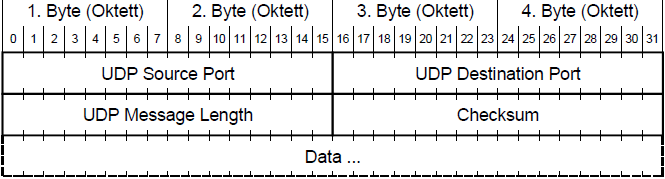
\includegraphics[height=2cm]{part3/UDP_Header}\end{verse}
\begin{itemize}
\item Source Port (16 Bits): Identifiziert sendende Appl. (0 wenn nichts
zurückkommen soll)
\item Destination Port (16 Bits): Identifiziert Appl. des Empfängers
\item Message Length (16 Bits): Länge des UDP Datagramms inkl. Header (in
Bytes) (Max. 65535 Bytes)
\item Checksum: Prüfsumme über Pseudo-Header, UDP Header und Daten.
\end{itemize}

\subsection*{Transmission Control Protocol (TCP)}

Soll unzuverlässiges IP erweitern um zuverlässigen Datentransport
zwischen Applikationen. Netze ROuter und Zielhost sollen nicht überlastet
werden.
\begin{itemize}
\item Verbindungsorientiert (End-zu-End Dienst, Verbindung ist virtuell:
wird nur durch Software hergestellt) 
\item Zuverlässiger Verbindungsaufsbau (beide Endpunkte müssen bestätigen)
\item Verbindungsaufbau über 3-Way-Handshake

\begin{itemize}
\item Anfrage Client: Seq=100, Ack=0, SYN
\item Bestätigung Server: Seq=200, Ack=101, SYN/ACK
\item Bestätigung Client: Seq=101, Ack=201, ACK
\end{itemize}
\item Hohe Zuverlässigkeit (Richtige Reihenfolge der Daten ohne Datenverlust)
\item Vollduplexübertragung
\item Stream-Schnittstelle
\item Eleganter Verbindungsabbau (Mit 4 Nachrichten; Zustellung aller Daten
auch dann, half Close)
\item Übertragung gekapselt in IP Paket (Router leiten weiter, IP-Modul
des Empfänger liefert es an das TCP-Modul weiter)
\item Umlaufverzögerung (Round Trip Delay) wird laufend gemessen und Wartezeit
bis Retransmission entsprechend eingestellt.
\end{itemize}

\subsubsection*{Sliding Window}
\begin{itemize}
\item Sender und Empfänger einigen sich auf fixe Fenstergrösse
\item Fenstergrösse = Maximale Paketmenge die ohne bestätigung gesendet
werden darf
\item Sender speichert jedes Paket bis zur bestätigung
\item Die Bestätigung enhält Anzahl offene Bytes im Fenster (Bei 0 gibts
später eine erneute bestätigung, das wieder Platz frei ist)
\end{itemize}

\subsubsection*{Congestion Control}

Überlastungsüberwachung (des Netzwerks), Congestion Window wird vom
Sender selbst ermittelt. Das kleinere der beiden Fenster (Congestion
oder Sliding) ist ausschlaggebend.
\begin{itemize}
\item Slow Start: Algorithmus zum ermitteln der Congestion Window grösse.
\item Beginnt mit Maximum Segment Size (MSS=1460 Bytes), bei Bestätigung
wirds verdoppelt
\item Ab einer bestimmten Schwelle (Threshold, Initial 64 KB) nimmt das
Fenster nur noch um 1 MSS zu
\item Bei einem Timout wird die Schwelle auf 1/2 des Congestion Window und
Congestion Window auf 1 MSS gesetzt.
\end{itemize}

\subsubsection*{TCP-Header}
\begin{verse}
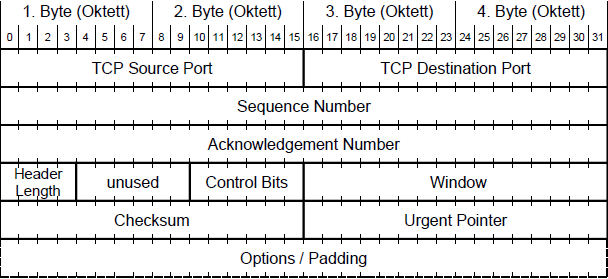
\includegraphics[height=4cm]{part3/TCP_Header}\end{verse}
\begin{itemize}
\item Source/Destination Port (je 16 Bits): Sender- und Empfängerport (bezeichnet
Applikation auf Serverseite)
\item Sequence Number (32 Bits): \end{itemize}

